\appendix \chapter{Appendix}
\label{chap:appendix}

\begin{algorithm}[language=NetLogo, caption={Interpersonal influence over trust}, label={algo:interpersonal}]
;; update agents' trust level when in contact with each other
to interpersonal-influence-over-trust
  ask turtles with [epidemic-state != "Hospitalised" and epidemic-state != "Deceased"] [
    let influencer-trust-level trust-level
    ask other turtles in-radius 0.1 with [epidemic-state != "Deceased"] [
      let proba-influ (ifelse-value
        ;; non-trusting agents are less influenced than trusting agents
        trust-level < 0.5 [ random-float trust-level / 0.5 ]
        [ random-float (1 - trust-level) + 0.5 ]
      )
      if random-float 1 < proba-influ
      [
        ;; influence trust
        (ifelse
          influencer-trust-level < 0.5
          [
            ;; influencer's trust level of 0.0 has an intensity of 1
            let influencer-influence-intensity 1 - (influencer-trust-level / 0.5)
            ;; high effectiveness on trust level 0.0 (low on 1.0)
            let influence-effectiveness 1 - trust-level
            let influence-update influencer-influence-intensity * influence-effectiveness
            set trust-level trust-level - influence-update
            if trust-level < 0 [ set trust-level 0 ]
          ]
          influencer-trust-level > 0.5
          [
            ;; influencer's trust level of 1.0 has an intensity of 1
            let influencer-influence-intensity (influencer-trust-level / 0.5) - 1
            ;; high effectiveness on trust level 1.0 (low on 0.0)
            let influence-effectiveness trust-level
            let influence-update influencer-influence-intensity * influence-effectiveness
            set trust-level trust-level + influence-update
            if trust-level > 1 [ set trust-level 1 ]
          ]
          ;; else influencer-trust-level == 0.5
          ;; influencer's trust level of 0.5 has an intensity of 0
        )
      ]
    ]
  ]
end
\end{algorithm}

\newpage

\begin{algorithm}[language=NetLogo, caption={Observational influence over trust}, label={algo:observational}]
;; update agents' trust level according to the infectious & vaccination status of agents around them (as well as themselves)
to observational-influence-over-trust
  if on-going-vaccination?
  [
    ask turtles with [epidemic-state != "Hospitalised" and epidemic-state != "Deceased"] [
      let observer-update 0
      ask other turtles in-radius 0.5 with [epidemic-state != "Deceased"] [
        let is-other-vaccinated? vaccinated?
        let is-other-symptomatic? ((epidemic-state = "Infected") or (epidemic-state = "Hospitalised"))
        ;; negative information have more impact than positive information
        (ifelse
          is-other-vaccinated? and (not is-other-symptomatic?)
          [
            ;; positive information
            set observer-update observer-update + (0.03 * trust-level)
          ]
          is-other-vaccinated? and is-other-symptomatic?
          [
            ;; negative information
            set observer-update observer-update - (0.05 * (1 - trust-level))
          ]
        )
      ]
      set trust-level trust-level + observer-update
      if trust-level < 0 [ set trust-level 0 ]
      if trust-level > 1 [ set trust-level 1 ]
    ]
  ]
end
\end{algorithm}

\newpage

\begin{algorithm}[language=NetLogo, caption={Institutional influence over trust}, label={algo:institutional}]
;; update agents' trust level comparing the percentage of agents in epidemiologic state X with the percentage of agents not in the epidemiologic state X
to institutional-influence-over-trust [nb-X nb-X-V is-X-D?]
  if on-going-vaccination? and nb-X > 0
  [
    ;; percentage of vaccinated among X
    let prop-X-V nb-to-prop nb-X-V nb-X
    ;; percentage of vaccinated not among X
    let prop-nX-V 0
    ifelse is-X-D?
      [set prop-nX-V nb-to-prop (total-vaccinations - nb-X-V) (population-size - nb-X)]
      [set prop-nX-V nb-to-prop (total-vaccinations - nb-X-V) (population-size - nb-X - nb-D)]
    ask turtles with [epidemic-state != "Hospitalised" and epidemic-state != "Deceased"] [
      let trust-level-update 0
      ;; institutional influence with a lack of knowledge or difficulties understanding statistics
      ifelse misinterpret? [
        set trust-level-update (prop-X-V / 100) * -1 * (1 - trust-level)
      ]
      ;; institutional influence with complete knowledge and understanding of statistics
      [
        let prop-nX-X-V-difference (prop-nX-V - prop-X-V) / 100

        ifelse prop-nX-X-V-difference >= 0 [
          ;; positive information is attenuated (* 0.5)
          ;; non-trusting agents will tend to neglect the positive information
          set trust-level-update prop-nX-X-V-difference * 0.5 * trust-level
        ]
        [
          ;; trusting agents will tend to neglect the negative information
          set trust-level-update prop-nX-X-V-difference * (1 - trust-level)
        ]
      ]
      set trust-level trust-level + trust-level-update
      if trust-level < 0 [ set trust-level 0 ]
      if trust-level > 1 [ set trust-level 1 ]
    ]
  ]
end
\end{algorithm}

\newpage

\begin{algorithm}[language=NetLogo, caption={Initialisation of the population's trust level}, label={algo:initialisation_trust_level}]
;; initialisation of each agent's trust level
to setup-population-trust-level
  ;; number of currently initialised agents' trust
  let current-trust-average-count 0
  ask turtles
  [
    (ifelse
      ;; if current population's average trust is below initial trust level
      ;; set trust level between X and 1
      ;; X = opposite number to current average of population trust based on initial trust level
      current-trust-average < initial-trust-level
      [
        let trust-average-adjuster (initial-trust-level + (initial-trust-level - current-trust-average))
        if trust-average-adjuster > 1
        [
          set trust-average-adjuster 0.9
        ]
        set trust-level trust-average-adjuster + (random-float (1 - trust-average-adjuster))
      ]
      ;; if current population's average trust is above initial trust level
      ;; set trust level between 0 and X
      ;; X = opposite number to current average of population trust based on initial trust level
      current-trust-average > initial-trust-level
      [
        let trust-average-adjuster (initial-trust-level - (current-trust-average - initial-trust-level))
        if trust-average-adjuster < 0
        [
          set trust-average-adjuster 0.1
        ]
        set trust-level random-float trust-average-adjuster
      ]
      ;; if current average of population trust is equal to initial trust level
      ;; set trust level between 0 and 1
      [
        set trust-level random-float 1
      ]
    )

    set current-trust-average-count current-trust-average-count + 1
    set current-trust-average (current-trust-average * (current-trust-average-count - 1) / current-trust-average-count + trust-level / current-trust-average-count)
  ]
end
\end{algorithm}

\newpage

\begin{figure}[!htb]
    \centering
    \minipage{\textwidth}
        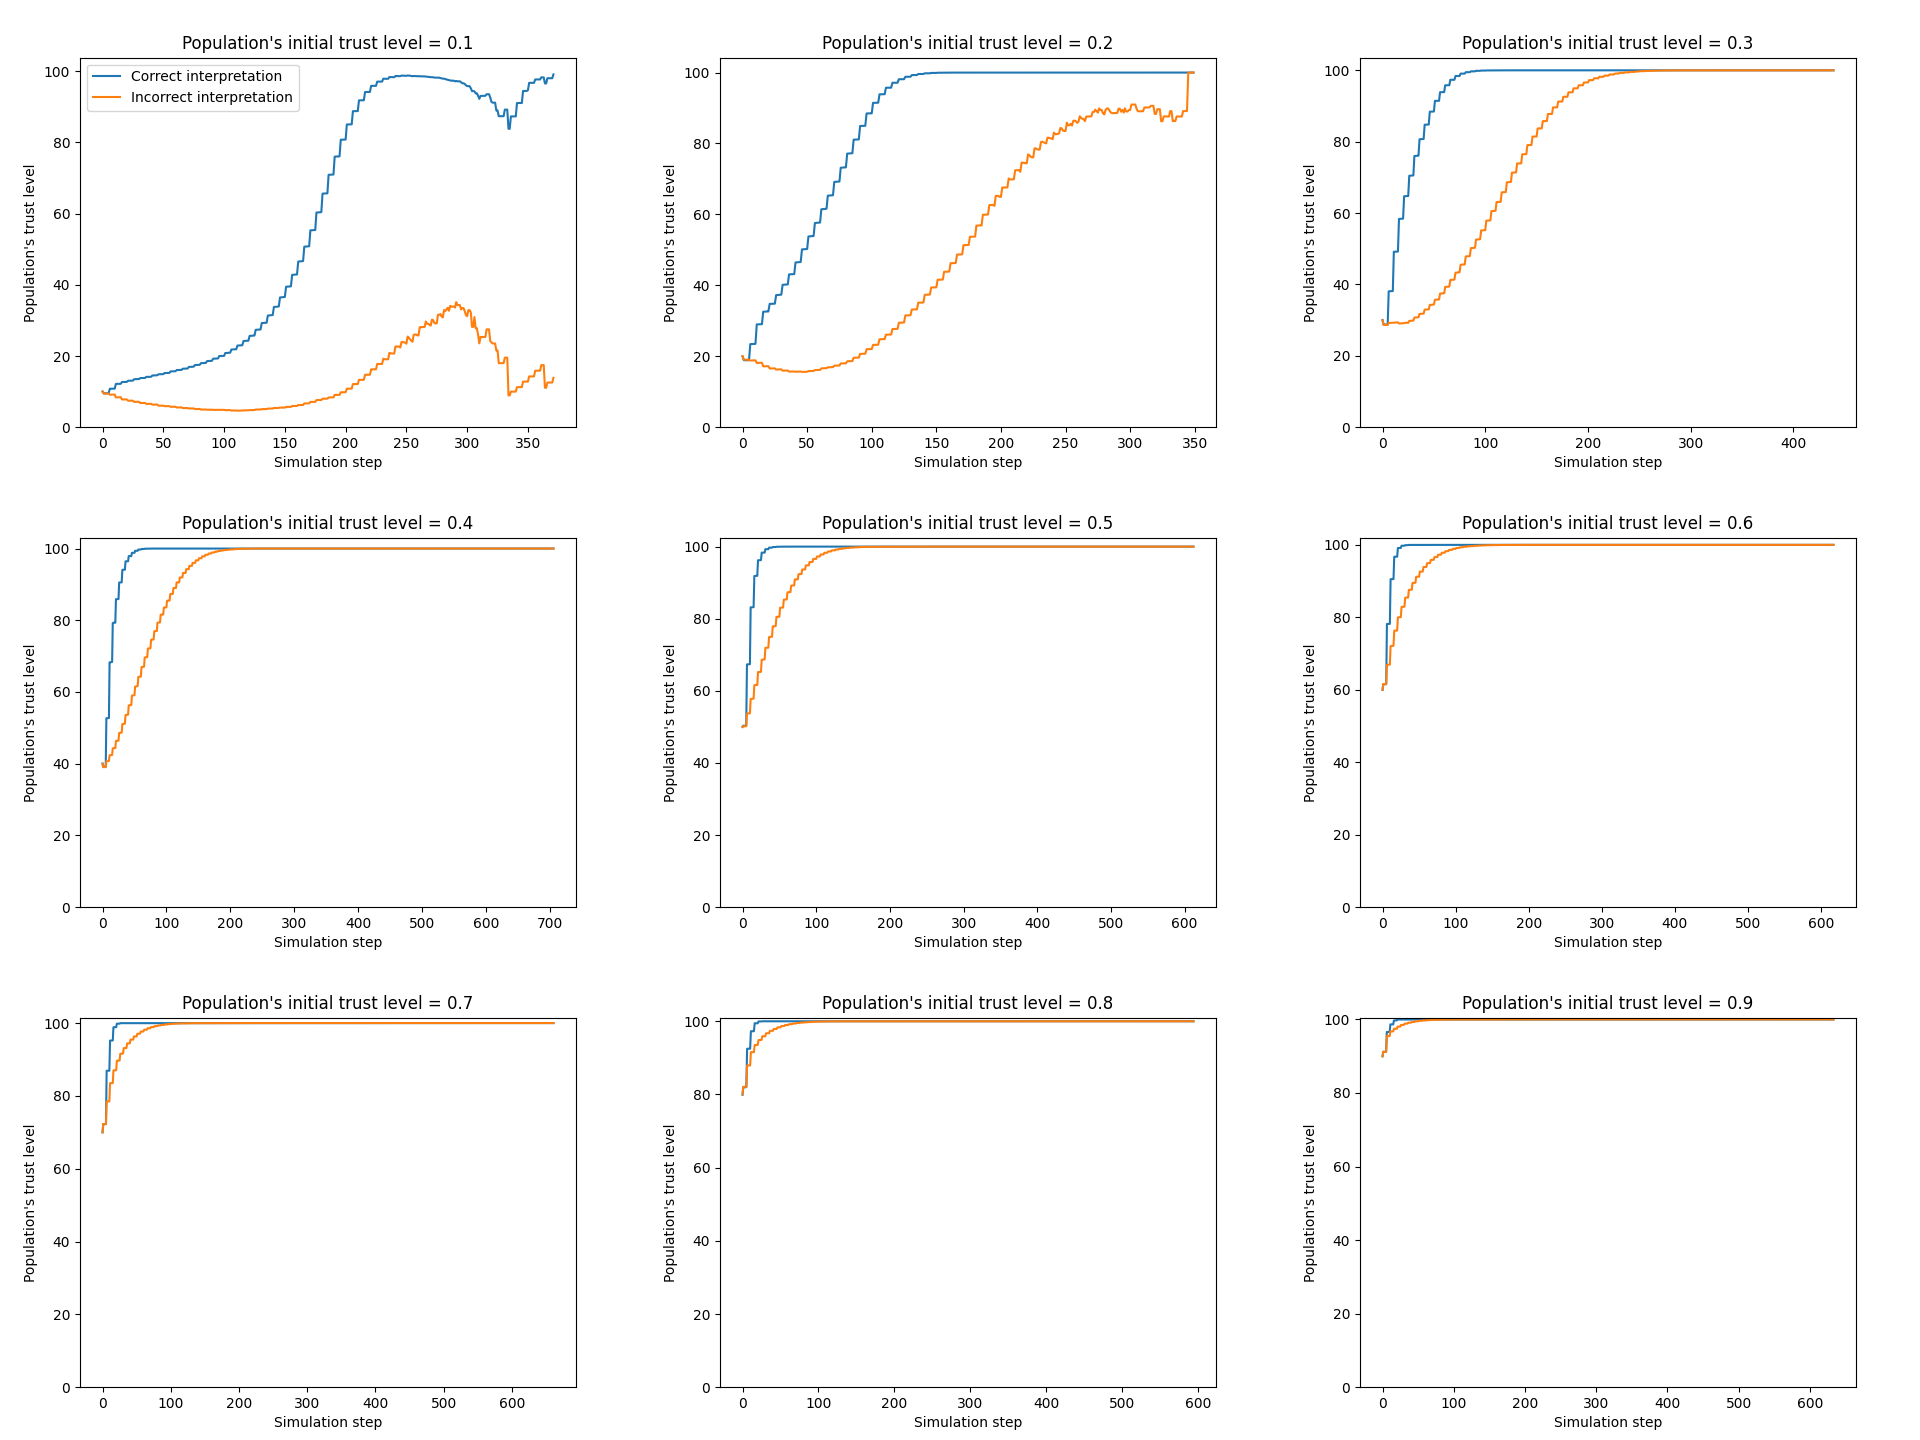
\includegraphics[width=1.3\linewidth, angle=90, origin=c]{pics/TM.png}
    \endminipage
    \caption{Average population's trust level per misinterpretation status at each simulation step for each population's initial trust level. The number of simulation steps (x-axis) is different between graphs.}
    \label{fig:tm_landscape}
\end{figure}

\newpage

\begin{figure}[!htb]
    \centering
    \minipage{\textwidth}
        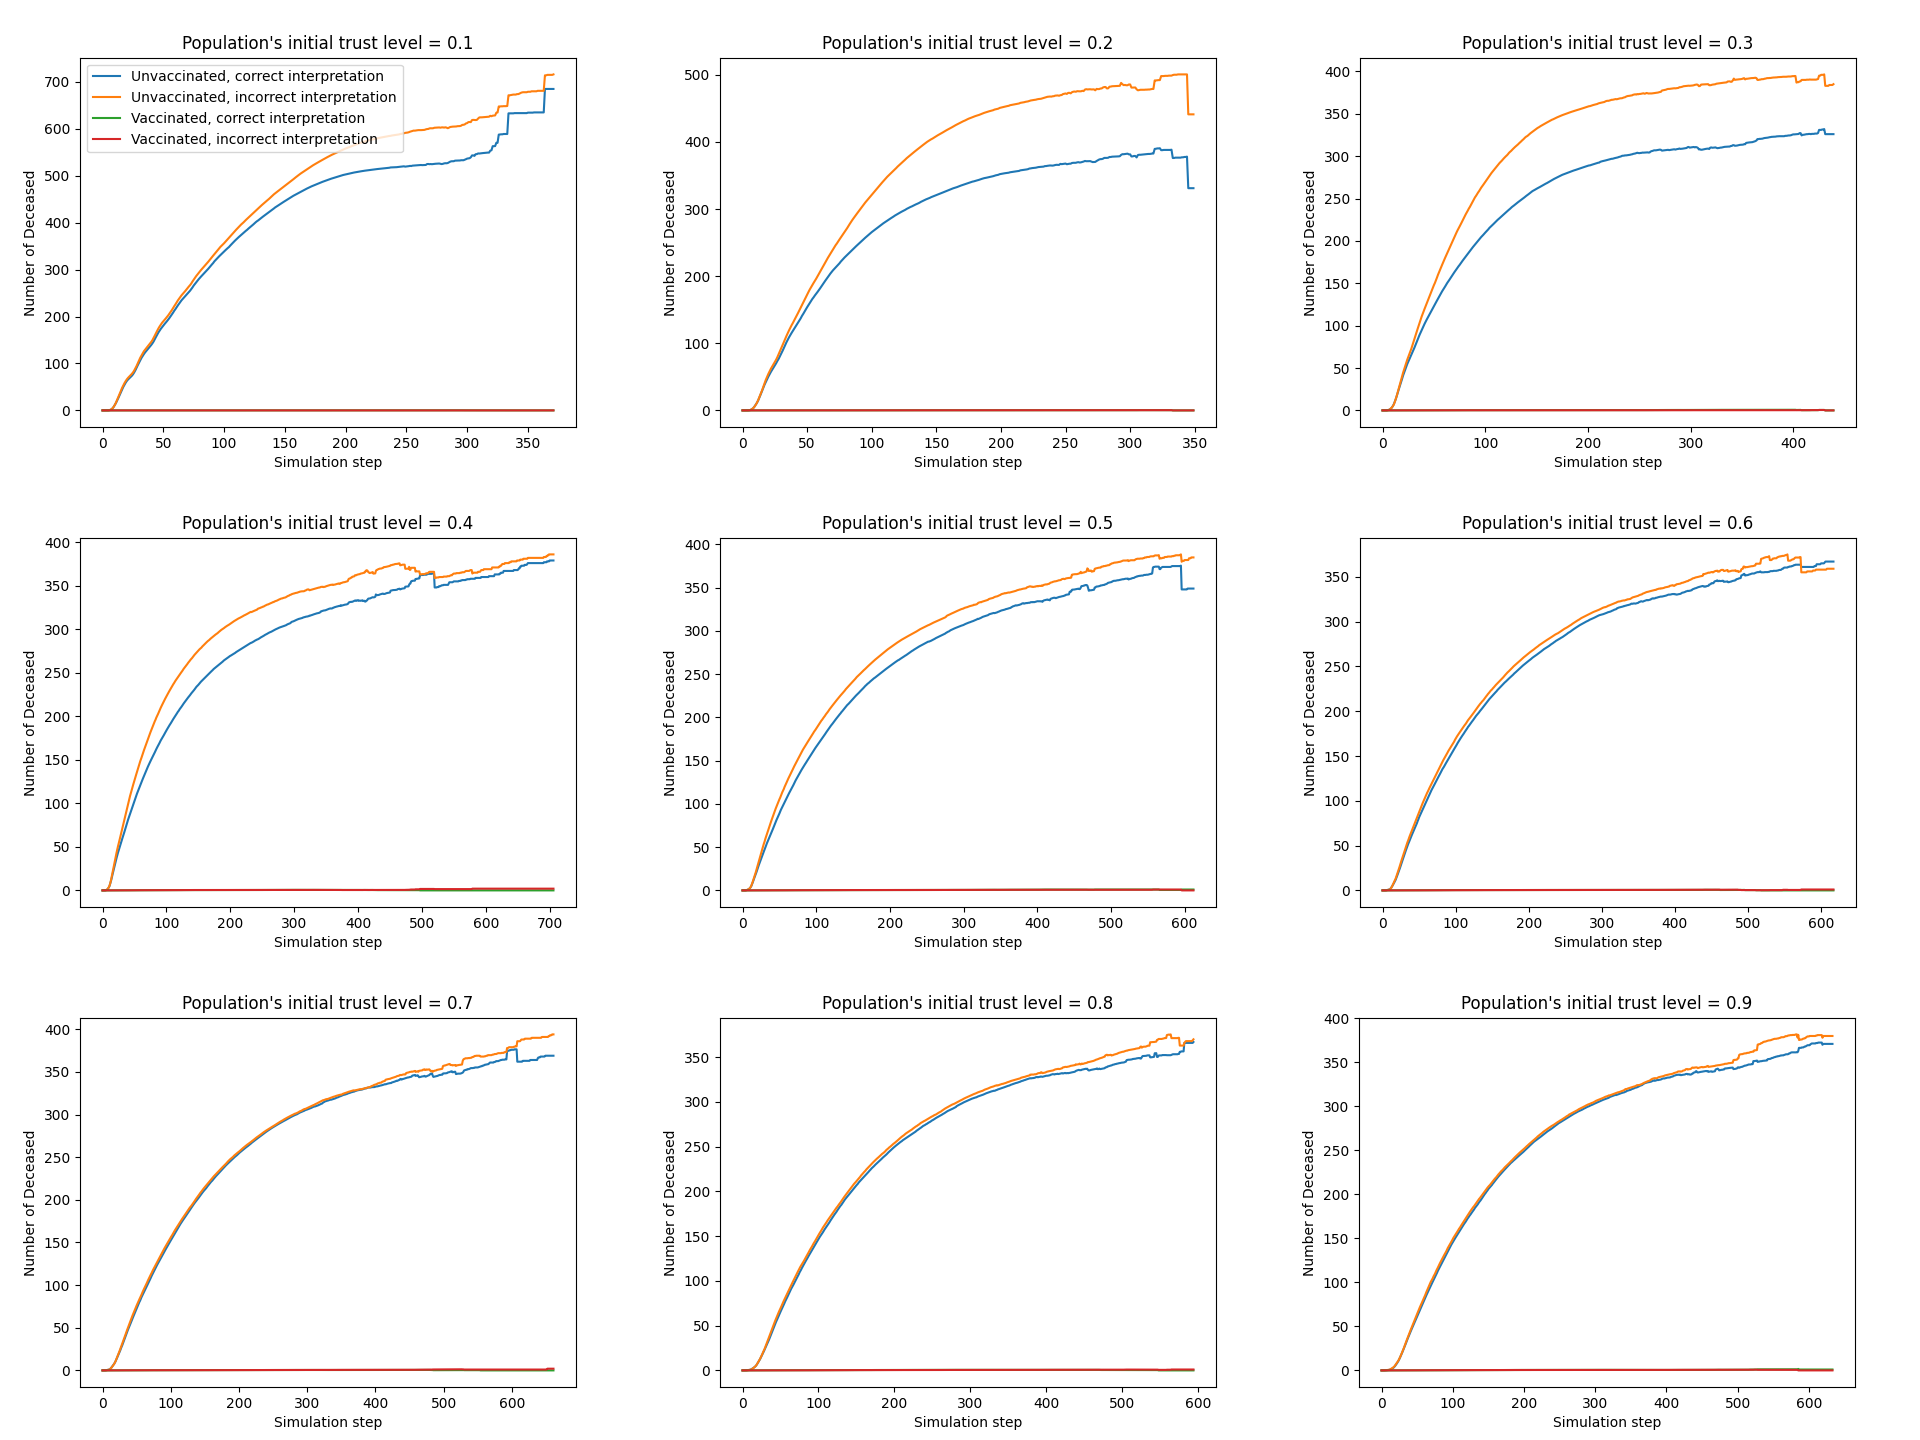
\includegraphics[width=1.3\linewidth, angle=90, origin=c]{pics/DVM.png}
    \endminipage
    \caption{Average number of deaths per vaccination and misinterpretation statuses at each simulation step for each population's initial trust level. The number of simulation steps (x-axis) is different between graphs.}
    \label{fig:dvm_landscape}
\end{figure}

\newpage

\begin{figure}[!htb]
    \centering
    \minipage{\textwidth}
        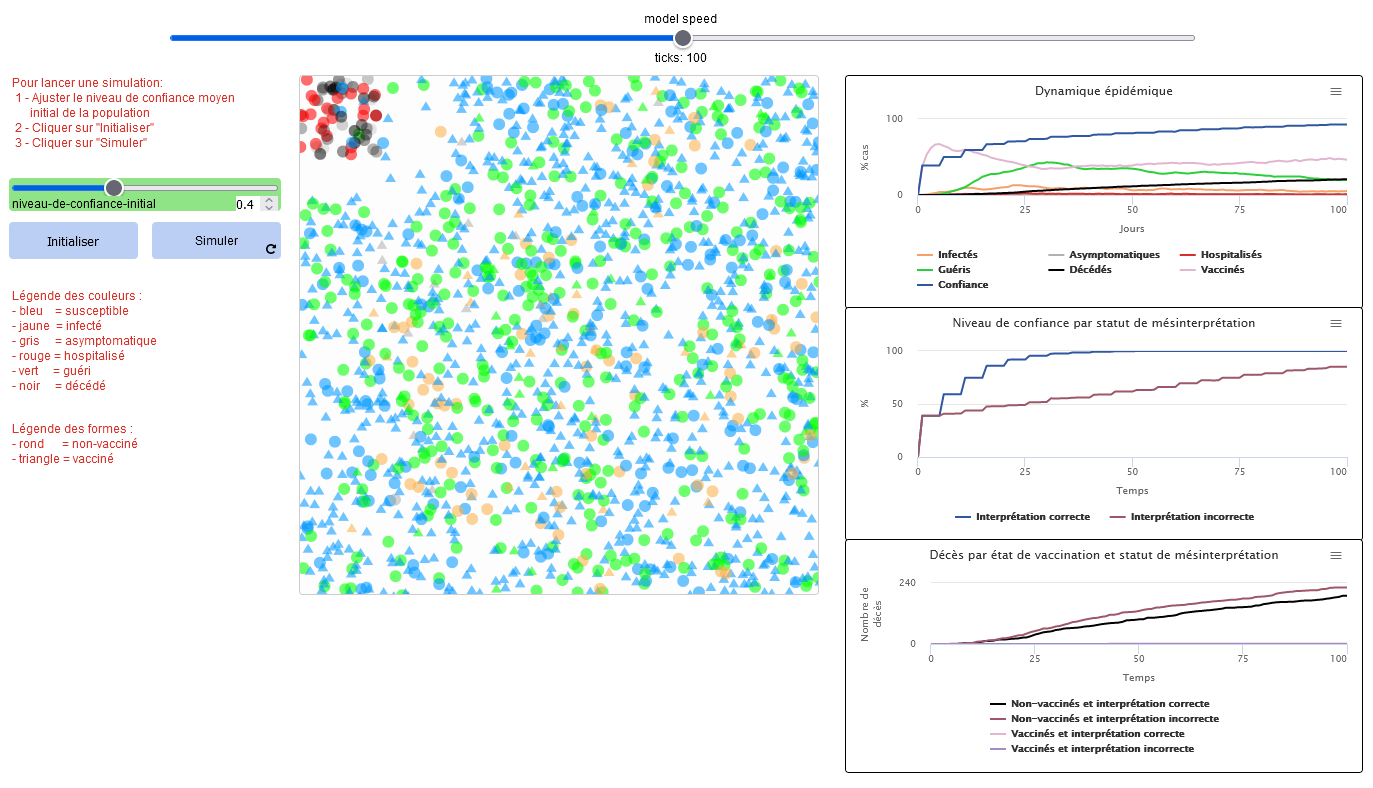
\includegraphics[width=1.4\linewidth, angle=90, origin=c]{pics/simulation_screenshot.png}
    \endminipage
    \caption{Screenshot of the simulation on NetLogo Web}
    \label{fig:simulation_screenshot}
\end{figure}

\newpage
